% Options for packages loaded elsewhere
\PassOptionsToPackage{unicode}{hyperref}
\PassOptionsToPackage{hyphens}{url}
%
\documentclass[
]{article}
\usepackage{lmodern}
\usepackage{amssymb,amsmath}
\usepackage{ifxetex,ifluatex}
\ifnum 0\ifxetex 1\fi\ifluatex 1\fi=0 % if pdftex
  \usepackage[T1]{fontenc}
  \usepackage[utf8]{inputenc}
  \usepackage{textcomp} % provide euro and other symbols
\else % if luatex or xetex
  \usepackage{unicode-math}
  \defaultfontfeatures{Scale=MatchLowercase}
  \defaultfontfeatures[\rmfamily]{Ligatures=TeX,Scale=1}
\fi
% Use upquote if available, for straight quotes in verbatim environments
\IfFileExists{upquote.sty}{\usepackage{upquote}}{}
\IfFileExists{microtype.sty}{% use microtype if available
  \usepackage[]{microtype}
  \UseMicrotypeSet[protrusion]{basicmath} % disable protrusion for tt fonts
}{}
\makeatletter
\@ifundefined{KOMAClassName}{% if non-KOMA class
  \IfFileExists{parskip.sty}{%
    \usepackage{parskip}
  }{% else
    \setlength{\parindent}{0pt}
    \setlength{\parskip}{6pt plus 2pt minus 1pt}}
}{% if KOMA class
  \KOMAoptions{parskip=half}}
\makeatother
\usepackage{xcolor}
\IfFileExists{xurl.sty}{\usepackage{xurl}}{} % add URL line breaks if available
\IfFileExists{bookmark.sty}{\usepackage{bookmark}}{\usepackage{hyperref}}
\hypersetup{
  pdftitle={Getting Started with Data in R},
  hidelinks,
  pdfcreator={LaTeX via pandoc}}
\urlstyle{same} % disable monospaced font for URLs
\usepackage[margin=1in]{geometry}
\usepackage{color}
\usepackage{fancyvrb}
\newcommand{\VerbBar}{|}
\newcommand{\VERB}{\Verb[commandchars=\\\{\}]}
\DefineVerbatimEnvironment{Highlighting}{Verbatim}{commandchars=\\\{\}}
% Add ',fontsize=\small' for more characters per line
\usepackage{framed}
\definecolor{shadecolor}{RGB}{248,248,248}
\newenvironment{Shaded}{\begin{snugshade}}{\end{snugshade}}
\newcommand{\AlertTok}[1]{\textcolor[rgb]{0.94,0.16,0.16}{#1}}
\newcommand{\AnnotationTok}[1]{\textcolor[rgb]{0.56,0.35,0.01}{\textbf{\textit{#1}}}}
\newcommand{\AttributeTok}[1]{\textcolor[rgb]{0.77,0.63,0.00}{#1}}
\newcommand{\BaseNTok}[1]{\textcolor[rgb]{0.00,0.00,0.81}{#1}}
\newcommand{\BuiltInTok}[1]{#1}
\newcommand{\CharTok}[1]{\textcolor[rgb]{0.31,0.60,0.02}{#1}}
\newcommand{\CommentTok}[1]{\textcolor[rgb]{0.56,0.35,0.01}{\textit{#1}}}
\newcommand{\CommentVarTok}[1]{\textcolor[rgb]{0.56,0.35,0.01}{\textbf{\textit{#1}}}}
\newcommand{\ConstantTok}[1]{\textcolor[rgb]{0.00,0.00,0.00}{#1}}
\newcommand{\ControlFlowTok}[1]{\textcolor[rgb]{0.13,0.29,0.53}{\textbf{#1}}}
\newcommand{\DataTypeTok}[1]{\textcolor[rgb]{0.13,0.29,0.53}{#1}}
\newcommand{\DecValTok}[1]{\textcolor[rgb]{0.00,0.00,0.81}{#1}}
\newcommand{\DocumentationTok}[1]{\textcolor[rgb]{0.56,0.35,0.01}{\textbf{\textit{#1}}}}
\newcommand{\ErrorTok}[1]{\textcolor[rgb]{0.64,0.00,0.00}{\textbf{#1}}}
\newcommand{\ExtensionTok}[1]{#1}
\newcommand{\FloatTok}[1]{\textcolor[rgb]{0.00,0.00,0.81}{#1}}
\newcommand{\FunctionTok}[1]{\textcolor[rgb]{0.00,0.00,0.00}{#1}}
\newcommand{\ImportTok}[1]{#1}
\newcommand{\InformationTok}[1]{\textcolor[rgb]{0.56,0.35,0.01}{\textbf{\textit{#1}}}}
\newcommand{\KeywordTok}[1]{\textcolor[rgb]{0.13,0.29,0.53}{\textbf{#1}}}
\newcommand{\NormalTok}[1]{#1}
\newcommand{\OperatorTok}[1]{\textcolor[rgb]{0.81,0.36,0.00}{\textbf{#1}}}
\newcommand{\OtherTok}[1]{\textcolor[rgb]{0.56,0.35,0.01}{#1}}
\newcommand{\PreprocessorTok}[1]{\textcolor[rgb]{0.56,0.35,0.01}{\textit{#1}}}
\newcommand{\RegionMarkerTok}[1]{#1}
\newcommand{\SpecialCharTok}[1]{\textcolor[rgb]{0.00,0.00,0.00}{#1}}
\newcommand{\SpecialStringTok}[1]{\textcolor[rgb]{0.31,0.60,0.02}{#1}}
\newcommand{\StringTok}[1]{\textcolor[rgb]{0.31,0.60,0.02}{#1}}
\newcommand{\VariableTok}[1]{\textcolor[rgb]{0.00,0.00,0.00}{#1}}
\newcommand{\VerbatimStringTok}[1]{\textcolor[rgb]{0.31,0.60,0.02}{#1}}
\newcommand{\WarningTok}[1]{\textcolor[rgb]{0.56,0.35,0.01}{\textbf{\textit{#1}}}}
\usepackage{graphicx,grffile}
\makeatletter
\def\maxwidth{\ifdim\Gin@nat@width>\linewidth\linewidth\else\Gin@nat@width\fi}
\def\maxheight{\ifdim\Gin@nat@height>\textheight\textheight\else\Gin@nat@height\fi}
\makeatother
% Scale images if necessary, so that they will not overflow the page
% margins by default, and it is still possible to overwrite the defaults
% using explicit options in \includegraphics[width, height, ...]{}
\setkeys{Gin}{width=\maxwidth,height=\maxheight,keepaspectratio}
% Set default figure placement to htbp
\makeatletter
\def\fps@figure{htbp}
\makeatother
\setlength{\emergencystretch}{3em} % prevent overfull lines
\providecommand{\tightlist}{%
  \setlength{\itemsep}{0pt}\setlength{\parskip}{0pt}}
\setcounter{secnumdepth}{-\maxdimen} % remove section numbering

\title{Getting Started with Data in R}
\author{}
\date{\vspace{-2.5em}}

\begin{document}
\maketitle

\emph{Seminar "Mastering your Data -- from Exploration to Visualization}

\hypertarget{getting-started}{%
\section{Getting Started with Data in R}\label{getting-started}}

Before we can start exploring data in R, there are some key concepts to
understand first:

\begin{enumerate}
\def\labelenumi{\arabic{enumi}.}
\tightlist
\item
  What are R and RStudio?
\item
  How do I code in R?
\item
  What are R packages?
\end{enumerate}

\hypertarget{what-are-r-and-rstudio}{%
\subsection{1. What are R and RStudio?}\label{what-are-r-and-rstudio}}

Throughout this book, we will assume that you are using R via RStudio.
First time users often confuse the two. At its simplest, R is like a
car's engine while RStudio is like a car's dashboard as illustrated here

\begin{figure}
\centering
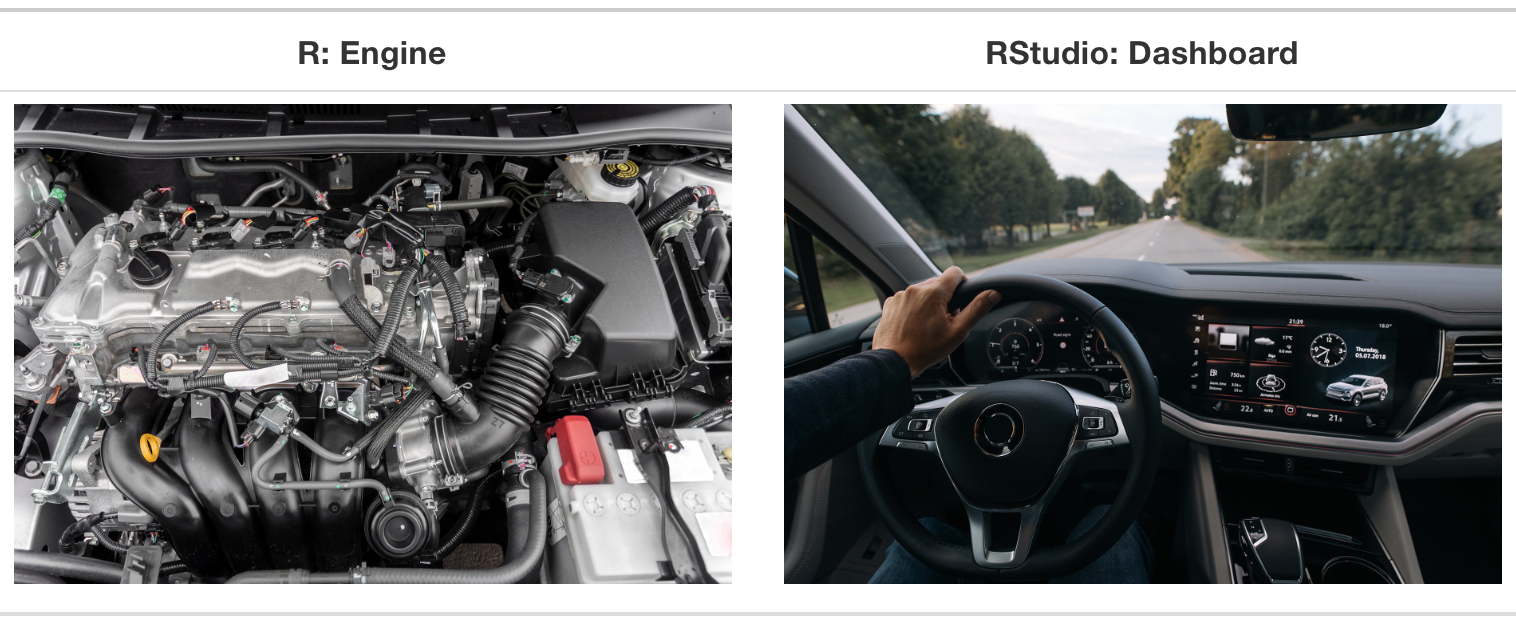
\includegraphics{../Figs/r_vs_rstudio_1.png}
\caption{Analogy of difference between R and RStudio.}
\end{figure}

More precisely, R is a programming language that runs computations,
while RStudio is an integrated development environment (IDE) that
provides an interface by adding many convenient features and tools. So
just as the way of having access to a speedometer, rearview mirrors, and
a navigation system makes driving much easier, using RStudio's interface
makes using R much easier as well.

\hypertarget{installing-r-and-rstudio}{%
\subsubsection{Installing R and
RStudio}\label{installing-r-and-rstudio}}

You will first need to download and install both R and RStudio (Desktop
version) on your computer. It is important that you install R first and
then install RStudio.

\begin{enumerate}
\def\labelenumi{\arabic{enumi}.}
\tightlist
\item
  \textbf{You must do this first:} Download and install R by going to
  \url{https://cloud.r-project.org/}. \index{R!installation}

  \begin{itemize}
  \tightlist
  \item
    If you are a Windows user: Click on ``Download R for Windows'', then
    click on ``base'', then click on the Download link.
  \item
    If you are macOS user: Click on ``Download R for (Mac) OS X'', then
    under ``Latest release:'' click on R-X.X.X.pkg, where R-X.X.X is the
    version number. For example, the latest version of R as of November
    25, 2019 was R-3.6.1.
  \item
    If you are a Linux user: Click on ``Download R for Linux'' and
    choose your distribution for more information on installing R for
    your setup.
  \end{itemize}
\item
  \textbf{You must do this second:} Download and install RStudio at
  \url{https://www.rstudio.com/products/rstudio/download/}.

  \begin{itemize}
  \tightlist
  \item
    Scroll down to ``Installers for Supported Platforms'' near the
    bottom of the page.
  \item
    Click on the download link corresponding to your computer's
    operating system.
  \end{itemize}
\end{enumerate}

\hypertarget{using-r-via-rstudio}{%
\subsubsection{Using R via RStudio}\label{using-r-via-rstudio}}

Recall our car analogy from earlier. Much as we don't drive a car by
interacting directly with the engine but rather by interacting with
elements on the car's dashboard, we won't be using R directly but rather
we will use RStudio's interface. After you install R and RStudio on your
computer, you'll have two new \emph{programs} (also called
\emph{applications}) you can open. We'll always work in RStudio and not
in the R application. Here shows what icon you should be clicking on
your computer.

\begin{figure}
\centering
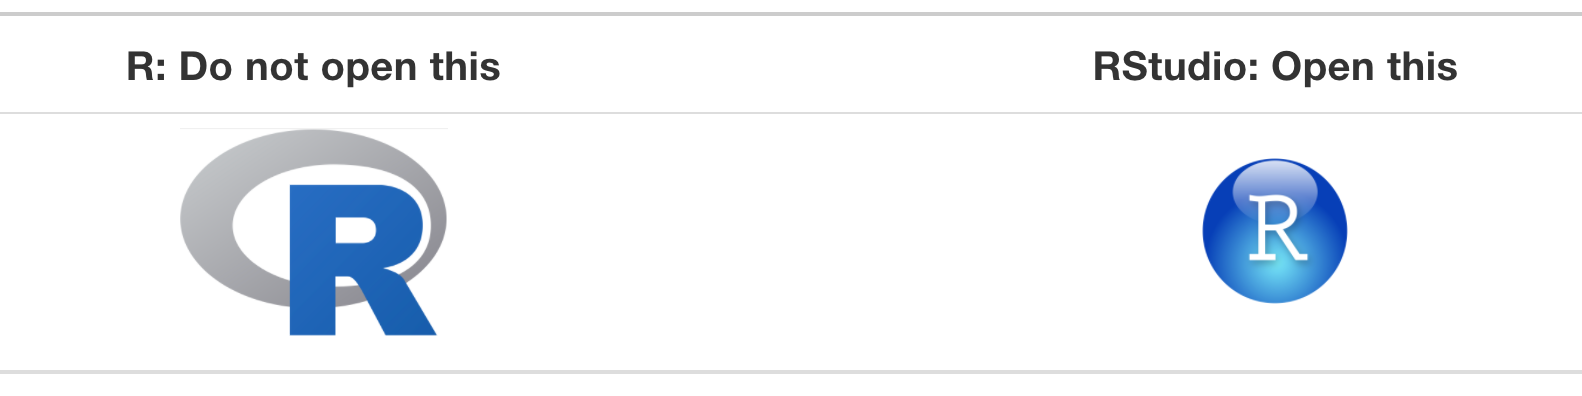
\includegraphics{../Figs/r_vs_rstudio.png}
\caption{Icons of R versus RStudio on your computer.}
\end{figure}

After you open RStudio, you should see something similar to this (Note
that slight differences might exist if the RStudio interface is updated
after 2019 to not be this by default.)
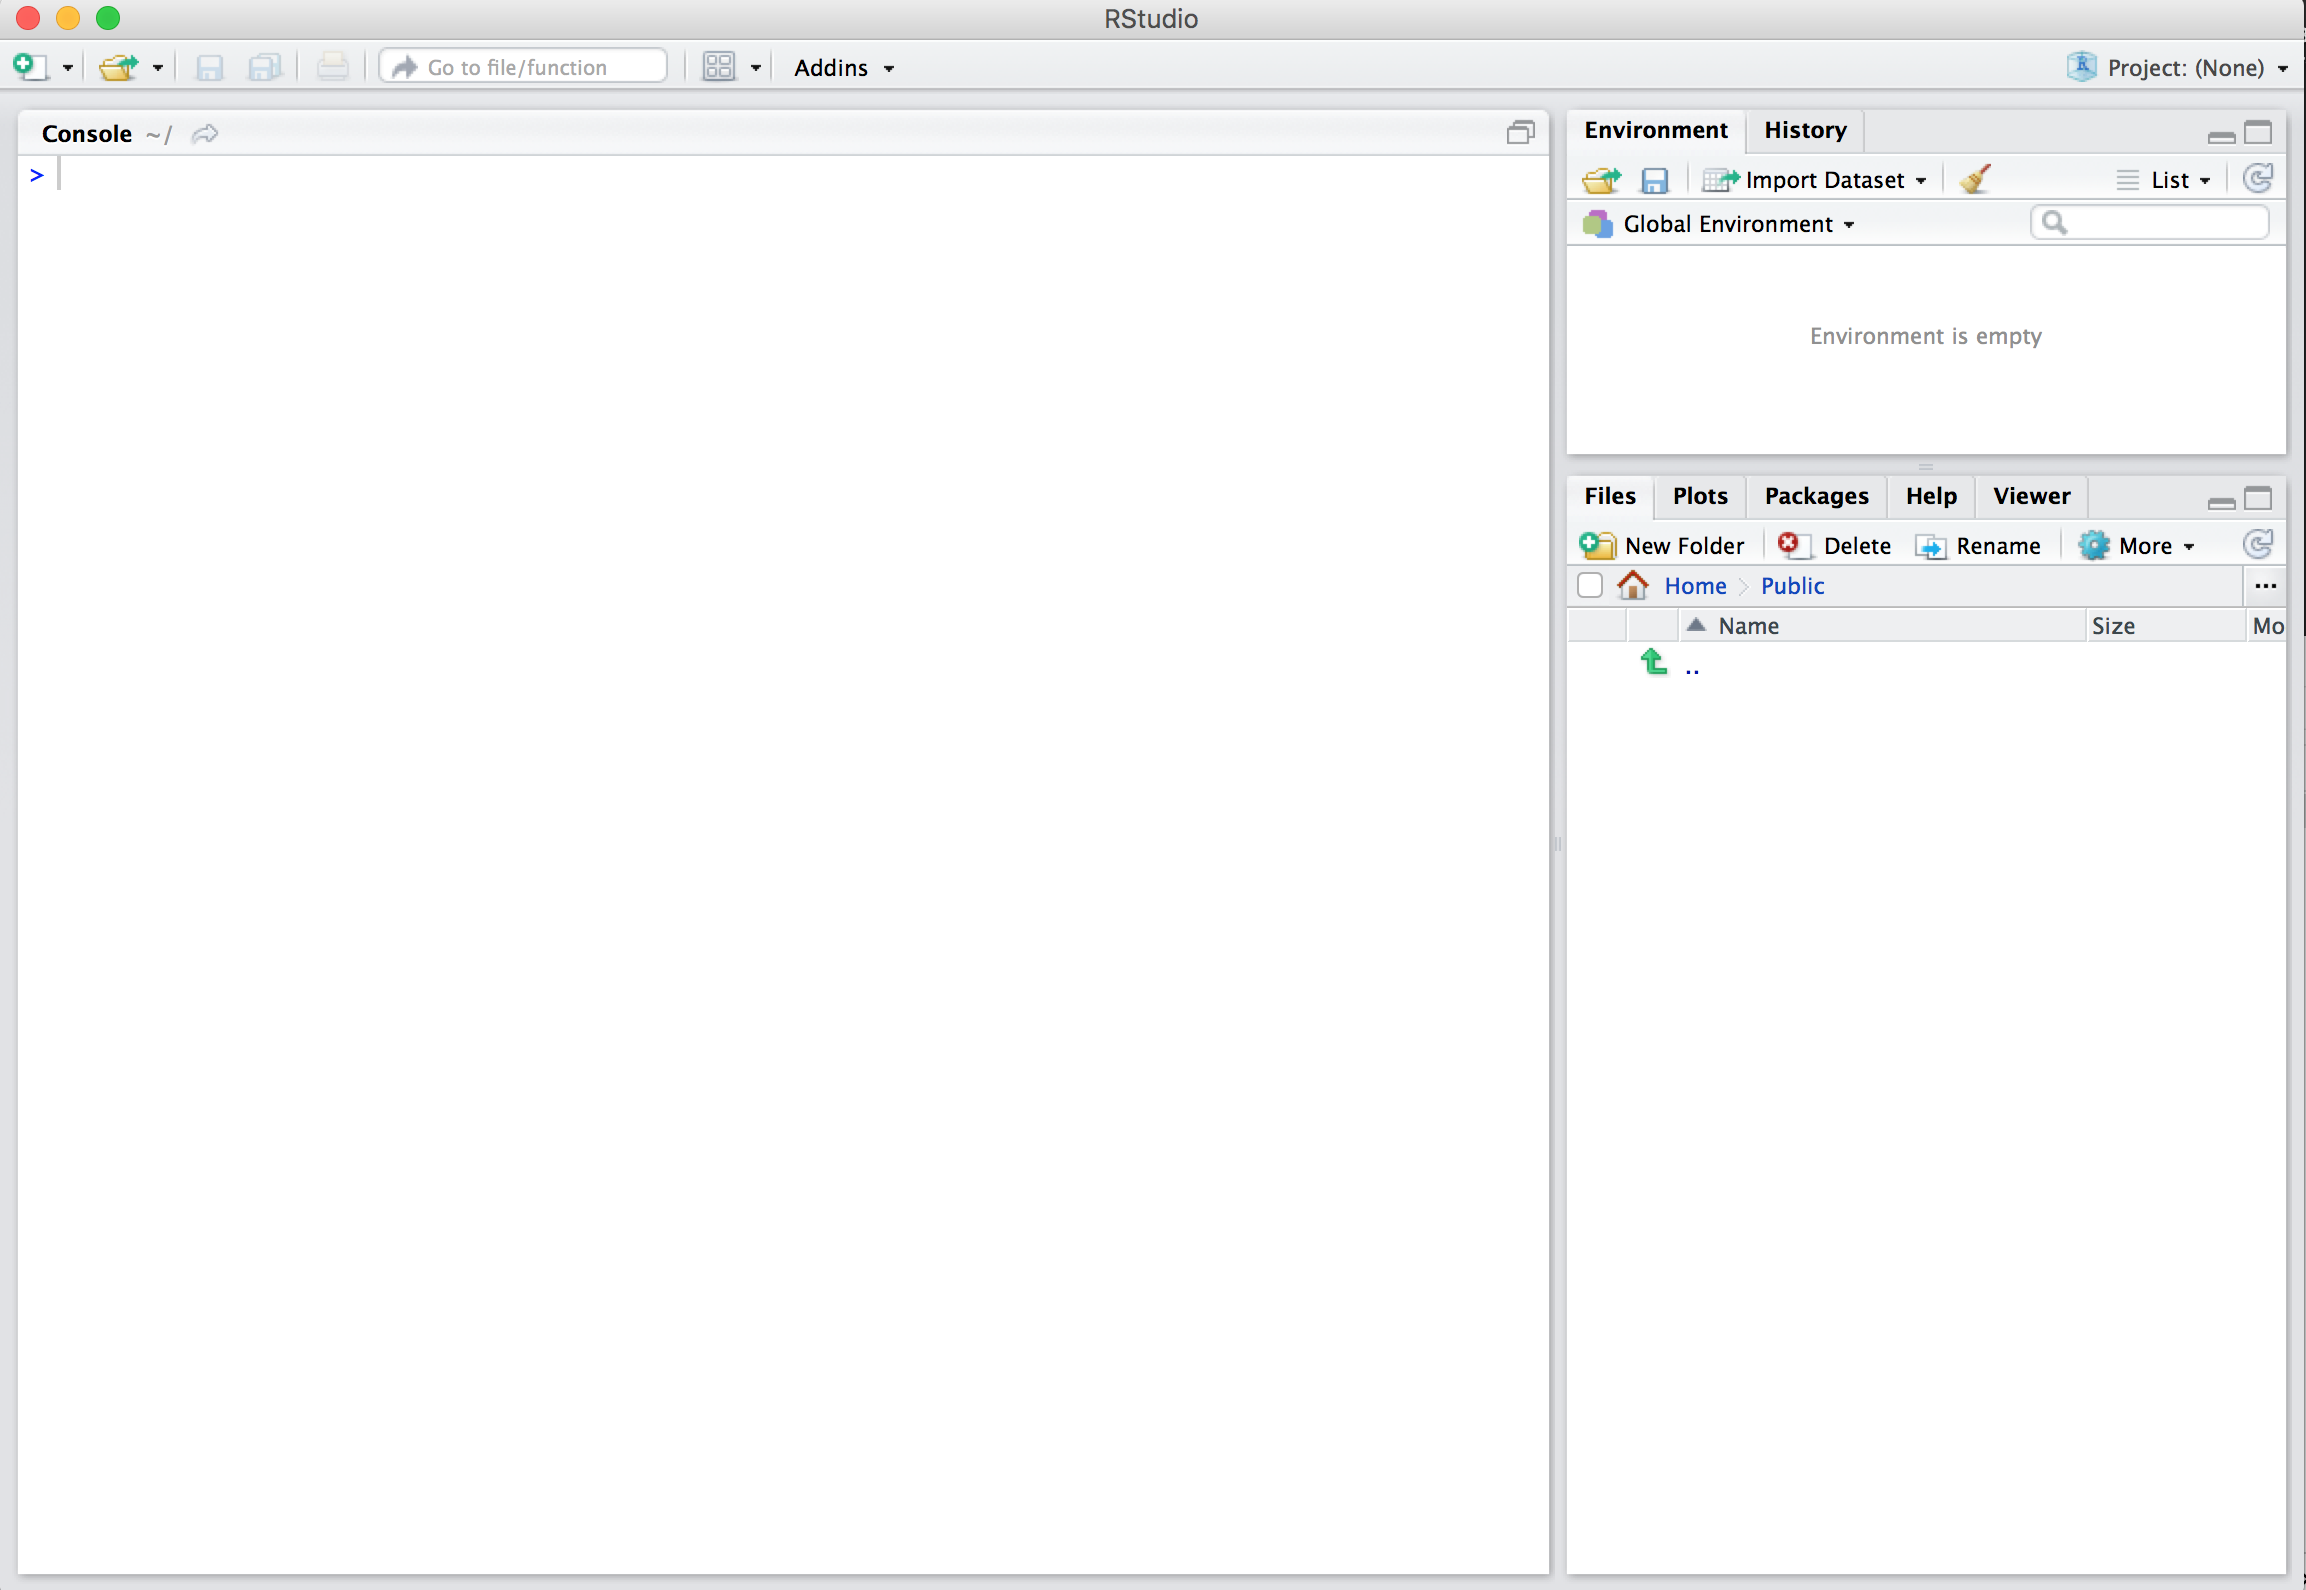
\includegraphics{../Figs/rstudio.png}

Note the three \emph{panes} which are three panels dividing the screen:
the \emph{console pane}, the \emph{files pane}, and the
\emph{environment pane}. Over the course of this chapter, you'll come to
learn what purpose each of these panes serves.

\hypertarget{code}{%
\subsection{How do I code in R?}\label{code}}

Now that you're set up with R and RStudio, you are probably asking
yourself, ``OK. Now how do I use R?''. The first thing to note is that
unlike other statistical software programs like Excel, SPSS, or Minitab
that provide
\href{https://en.wikipedia.org/wiki/Point_and_click}{point-and-click}
interfaces, R is an
\href{https://en.wikipedia.org/wiki/Interpreted_language}{interpreted
language}. This means you have to type in commands written in \emph{R
code}. In other words, you have to code/program in R. Note that we'll
use the terms ``coding'' and ``programming'' interchangeably in this
book.

While it is not required to be a seasoned coder/computer programmer to
use R, there is still a set of basic programming concepts that new R
users need to understand. Consequently, while this book is not a book on
programming, you will still learn just enough of these basic programming
concepts needed to explore and analyze data effectively.

\hypertarget{programming-concepts}{%
\subsubsection{Basic programming concepts and
terminology}\label{programming-concepts}}

We now introduce some basic programming concepts and terminology.
Instead of asking you to memorize all these concepts and terminology
right now, we'll guide you so that you'll ``learn by doing.'' To help
you learn, we will always use a different font to distinguish regular
text from \texttt{computer\_code}. The best way to master these topics
is, in our opinions, through
\href{https://jamesclear.com/deliberate-practice-theory}{deliberate
practice} with R and lots of repetition.

\begin{itemize}
\tightlist
\item
  Basics:

  \begin{itemize}
  \tightlist
  \item
    \emph{Console pane}: where you enter in commands.
  \item
    \emph{Running code}: the act of telling R to perform an act by
    giving it commands in the console.
  \item
    \emph{Objects}: where values are saved in R. We'll show you how to
    \emph{assign} values to objects and how to display the contents of
    objects. \index{objects}
  \item
    \emph{Data types}: integers, doubles/numerics, logicals, and
    characters. \index{data types} Integers are values like -1, 0, 2,
    4092. Doubles or numerics are a larger set of values containing both
    the integers but also fractions and decimal values like -24.932 and
    0.8. Logicals are either \texttt{TRUE} or \texttt{FALSE} while
    characters are text such as ``cancer'', ``hospital'', ``The patient
    comes from the city hospital'', and ``My name is Peter.'' Note that
    characters are often denoted with the quotation marks around them.
  \end{itemize}
\item
  \emph{Vectors}: a series of values.
\item
  \emph{Factors}: \emph{categorical data} are commonly represented in R
  as factors. Categorical data can also be represented as
  \emph{strings}.
\item
  \emph{Data frames}: rectangular spreadsheets. They are representations
  of datasets in R where the rows correspond to \emph{observations} and
  the columns correspond to \emph{variables} that describe the
  observations.
\end{itemize}

If you have worked with a spreadsheet such as Excel think the dataframe
as the spreadsheet and vectors as the columns.

\hypertarget{messages}{%
\subsubsection{Errors, warnings, and messages}\label{messages}}

One thing that intimidates new R and RStudio users is how it reports
\emph{errors}, \emph{warnings}, and \emph{messages}. R reports errors,
warnings, and messages in a glaring red font, which makes it seem like
it is scolding you. However, seeing red text in the console is not
always bad.

R will show red text in the console pane in three different situations:

\begin{itemize}
\tightlist
\item
  \textbf{Errors}: \index{R!errors} When the red text is a legitimate
  error, it will be prefaced with ``Error in\ldots{}'' and will try to
  explain what went wrong. Generally when there's an error, the code
  will not run. For example, we'll see in Subsection @ref(package-use)
  if you see
  \texttt{Error\ in\ ggplot(...)\ :\ could\ not\ find\ function\ "ggplot"},
  it means that the \texttt{ggplot()} function is not accessible because
  the package that contains the function (\texttt{ggplot2}) was not
  loaded with \texttt{library(ggplot2)}. Thus you cannot use the
  \texttt{ggplot()} function without the \texttt{ggplot2} package being
  loaded first.
\item
  \textbf{Warnings}: \index{R!warnings} When the red text is a warning,
  it will be prefaced with ``Warning:'' and R will try to explain why
  there's a warning. Generally your code will still work, but with some
  caveats. For example, you will see in Chapter @ref(viz) if you create
  a scatterplot based on a dataset where two of the rows of data have
  missing entries that would be needed to create points in the
  scatterplot, you will see this warning:
  \texttt{Warning:\ Removed\ 2\ rows\ containing\ missing\ values\ (geom\_point)}.
  R will still produce the scatterplot with all the remaining
  non-missing values, but it is warning you that two of the points
  aren't there.
\item
  \textbf{Messages}: \index{R!messages} When the red text doesn't start
  with either ``Error'' or ``Warning'', it's \emph{just a friendly
  message}. You'll see these messages when you load \emph{R packages} in
  the upcoming Subsection @ref(package-loading) or when you read data
  saved in spreadsheet files with the \texttt{read\_csv()} function as
  you'll see in Chapter @ref(tidy). These are helpful diagnostic
  messages and they don't stop your code from working. Additionally,
  you'll see these messages when you install packages too using
  \texttt{install.packages()} as discussed in Subsection
  @ref(package-installation).
\end{itemize}

Remember, when you see red text in the console, \emph{don't panic}. It
doesn't necessarily mean anything is wrong. Rather:

\begin{itemize}
\tightlist
\item
  If the text starts with ``Error'', figure out what's causing it.
  {Think of errors as a red traffic light: something is wrong!}
\item
  If the text starts with ``Warning'', figure out if it's something to
  worry about. For instance, if you get a warning about missing values
  in a scatterplot and you know there are missing values, you're fine.
  If that's surprising, look at your data and see what's missing. {Think
  of warnings as a yellow traffic light: everything is working fine, but
  watch out/pay attention.}
\item
  Otherwise, the text is just a message. Read it, wave back at R, and
  thank it for talking to you. {Think of messages as a green traffic
  light: everything is working fine and keep on going!}
\end{itemize}

\hypertarget{tips-code}{%
\subsubsection{Tips on learning to code}\label{tips-code}}

Learning to code/program is quite similar to learning a foreign
language. It can be daunting and frustrating at first. Such frustrations
are common and it is normal to feel discouraged as you learn. However,
just as with learning a foreign language, if you put in the effort and
are not afraid to make mistakes, anybody can learn and improve.

Here are a few useful tips to keep in mind as you learn to program:

\begin{itemize}
\tightlist
\item
  \textbf{Remember that computers are not actually that smart}: You may
  think your computer or smartphone is ``smart,'' but really people
  spent a lot of time and energy designing them to appear ``smart.'' In
  reality, you have to tell a computer everything it needs to do.
  Furthermore, the instructions you give your computer can't have any
  mistakes in them, nor can they be ambiguous in any way.
\item
  \textbf{Take the ``copy, paste, and tweak'' approach}: Especially when
  you learn your first programming language or you need to understand
  particularly complicated code, it is often much easier to take
  existing code that you know works and modify it to suit your ends.
  This is as opposed to trying to type out the code from scratch. We
  call this the \emph{``copy, paste, and tweak''} approach. So early on,
  we suggest not trying to write code from memory, but rather take
  existing examples we have provided you, then copy, paste, and tweak
  them to suit your goals. After you start feeling more confident, you
  can slowly move away from this approach and write code from scratch.
  Think of the ``copy, paste, and tweak'' approach as training wheels
  for a child learning to ride a bike. After getting comfortable, they
  won't need them anymore.
\item
  \textbf{The best way to learn to code is by doing}: Rather than
  learning to code for its own sake, we find that learning to code goes
  much smoother when you have a goal in mind or when you are working on
  a particular project, like analyzing data that you are interested in
  and that is important to you.
\item
  \textbf{Practice is key}: Just as the only method to improve your
  foreign language skills is through lots of practice and speaking, the
  only method to improving your coding skills is through lots of
  practice. Don't worry, however, we'll give you plenty of opportunities
  to do so!
\end{itemize}

\hypertarget{packages}{%
\subsection{What are R packages?}\label{packages}}

Another point of confusion with many new R users is the idea of an R
package. R packages extend the functionality of R by providing
additional functions, data, and documentation. They are written by a
worldwide community of R users and can be downloaded for free from the
internet.

For example, among the many packages we will use in this book are the
\texttt{ggplot2} package, the \texttt{dplyr} package for data wrangling
and many others. There are some packages that include several other
packages. This is the case with \texttt{tidyverse}, which includes many
of the packages needed for the usual data science tasks

A good analogy for R packages is they are like apps you can download
onto a mobile phone:

\begin{figure}
\centering
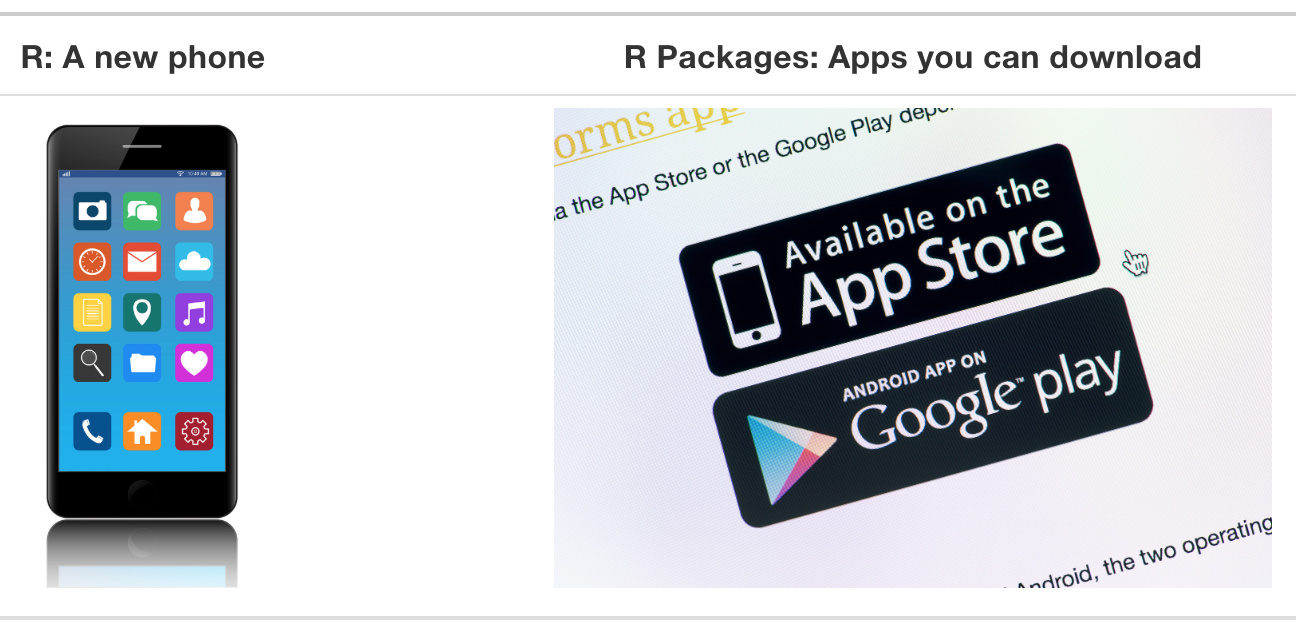
\includegraphics{../Figs/r_vs_r_packages.png}
\caption{Analogy of R versus R packages.}
\end{figure}

So R is like a new mobile phone: while it has a certain amount of
features when you use it for the first time, it doesn't have everything.
R packages are like the apps you can download onto your phone from
Apple's App Store or Android's Google Play.

Let's continue this analogy by considering the Instagram app for editing
and sharing pictures. Say you have purchased a new phone and you would
like to share a photo you have just taken with friends on Instagram. You
need to:

\begin{enumerate}
\def\labelenumi{\arabic{enumi}.}
\tightlist
\item
  \emph{Install the app}: Since your phone is new and does not include
  the Instagram app, you need to download the app from either the App
  Store or Google Play. You do this once and you're set for the time
  being. You might need to do this again in the future when there is an
  update to the app.
\item
  \emph{Open the app}: After you've installed Instagram, you need to
  open it.
\end{enumerate}

Once Instagram is open on your phone, you can then proceed to share your
photo with your friends and family. The process is very similar for
using an R package. You need to:

\begin{enumerate}
\def\labelenumi{\arabic{enumi}.}
\tightlist
\item
  \emph{Install the package}: This is like installing an app on your
  phone. Most packages are not installed by default when you install R
  and RStudio. Thus if you want to use a package for the first time, you
  need to install it first. Once you've installed a package, you likely
  won't install it again unless you want to update it to a newer
  version.
\item
  \emph{``Load'' the package}: ``Loading'' a package is like opening an
  app on your phone. Packages are not ``loaded'' by default when you
  start RStudio on your computer; you need to ``load'' each package you
  want to use every time you start RStudio.
\end{enumerate}

Let's perform these two steps for the \texttt{tidyverse} package that
includes many other packages, as `ggplot2' data visualization.

\hypertarget{package-installation}{%
\subsubsection{Package installation}\label{package-installation}}

\begin{enumerate}
\def\labelenumi{\alph{enumi})}
\tightlist
\item
  Click on the ``Packages'' tab.
\item
  Type the name of the package under ``Packages (separate multiple with
  space or comma):'' In this case, type \texttt{tidyverse}.
\item
  Click on ``Install'' next to Update.
\item
  Click ``Install.''
\end{enumerate}

\begin{figure}
\centering
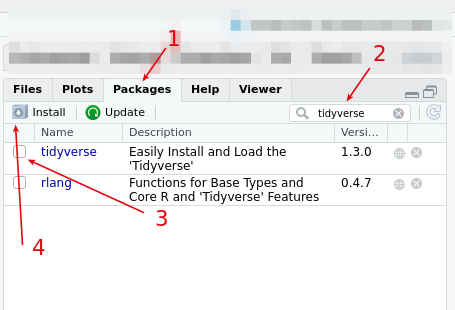
\includegraphics{../Figs/tidyverse01.png}
\caption{``Tidyverse package installation''}
\end{figure}

An alternative but slightly less convenient way to install a package is
by typing \texttt{install.packages("tidyverse")} in the console pane of
RStudio and pressing Return/Enter on your keyboard. Note you must
include the quotation marks around the name of the package.

Much like an app on your phone, you only have to install a package once.
However, if you want to update a previously installed package to a newer
version, you need to reinstall it by repeating the earlier steps.

Repeat the earlier installation steps, but for the
\texttt{palmerpenguins}, \texttt{NHANES}, and \texttt{janitor} packages.
This will install the earlier mentioned packages. We'll use these
packages (and more) during the course.

Note that if you'd like your output on your computer to match up exactly
with the output presented throughout the book, you may want to use the
exact versions of the packages that we used. You can find a full listing
of these packages and their versions in Appendix @ref(appendixE). This
likely won't be relevant for novices, but we included it for
reproducibility reasons.

\hypertarget{package-loading}{%
\subsubsection{Package loading}\label{package-loading}}

Recall that after you've installed a package, you need to ``load it.''
In other words, you need to ``open it.'' We do this by using the
\texttt{library()} command. \index{R packages!loading}

For example, to load the \texttt{ggplot2} package, run the following
code in the console pane. What do we mean by ``run the following code''?
Either type or copy-and-paste the following code into the console pane
and then hit the Enter key.

\begin{Shaded}
\begin{Highlighting}[]
\KeywordTok{library}\NormalTok{(ggplot2)}
\end{Highlighting}
\end{Shaded}

If after running the earlier code, a blinking cursor returns next to the
\texttt{\textgreater{}} ``prompt'' sign, it means you were successful
and the \texttt{ggplot2} package is now loaded and ready to use. If,
however, you get a red ``error message'' that reads \texttt{...}

\begin{verbatim}
Error in library(ggplot2) : there is no package called ‘ggplot2’
\end{verbatim}

\texttt{...} it means that you didn't successfully install it. This is
an example of an ``error message'' . If you get this error message, go
back to of Package Installation on R package installation and make sure
to install the \texttt{tidyverse} package before proceeding.

\hypertarget{package-use}{%
\subsubsection{Package use}\label{package-use}}

One very common mistake new R users make when wanting to use particular
packages is they forget to ``load'' them first by using the
\texttt{library()} command we just saw. Remember: \emph{you have to load
each package you want to use every time you start RStudio.} If you don't
first ``load'' a package, but attempt to use one of its features, you'll
see an error message similar to:

\begin{verbatim}
Error: could not find function
\end{verbatim}

This is a different error message than the one you just saw on a package
not having been installed yet. R is telling you that you are trying to
use a function in a package that has not yet been ``loaded.'' R doesn't
know where to find the function you are using. Almost all new users
forget to do this when starting out, and it is a little annoying to get
used to doing it. However, you'll remember with practice and after some
time it will become second nature for you.

\end{document}
